\documentclass[12pt,a4paper]{article}
\usepackage{apacite}
\usepackage{graphicx}
\usepackage[top=4cm, bottom=4cm, outer=5cm, inner=3cm, heightrounded, marginparwidth=3cm, marginparsep=1cm]{geometry} %TODO: comment out
%\usepackage[marginparwidth=2.5cm, marginparsep=2cm]{geometry}
\usepackage[toc,page]{appendix}
\usepackage{hyperref}
\usepackage{fancyref}
\usepackage[round]{natbib}
\usepackage{fancyhdr}
\usepackage{setspace}
\usepackage[justification=centering]{caption}
\pagestyle{fancy}

\newcommand{\citetwo}[4]{(\citeauthor{#1}, \citeyear{#1}, p.~#2; \citeauthor{#3}, \citeyear{#3}, p.~#4)}

\newcommand{\HRule}{\rule{\linewidth}{0.5mm}}



\begin{document}

\begin{titlepage}

\begin{center}

\textsc{\LARGE University of Edinburgh}\\[1cm]

\textsc{\Large Dissertation in Language Sciences}\\[1.5cm]

\HRule \\[0.4cm]
{ \huge \bfseries Understanding Referential Coordination as a Particle Swarm Optimization Task \\[0.4cm] }

\HRule \\[1.5cm]


\noindent
\begin{minipage}{0.4\textwidth}
\begin{flushleft} \large
\emph{Exam Number:}\\
---
\end{flushleft}
\end{minipage}%
\begin{minipage}{0.4\textwidth}
\begin{flushright} \large
\emph{Supervisor:} \\
Dr.~Hannah \textsc{Rohde}
\end{flushright}
\end{minipage}

\vfill

% Bottom of the page
{\large 1st April, 2015}
%\title{Understanding Referential Coordination as a Particle Swarm Optimization Task}
%\author{s1107496}
%\date{1st April, 2015}

%\maketitle

\end{center}
\end{titlepage}

\onehalfspace
%\doublespace

\begin{abstract}
% TODO: reverse structure (problem first, then PSO)
Particle swarm optimization (PSO) has been proposed as a means of modeling changes in human behaviour in a social context. PSO has also been shown to be an effective optimization method for non-differentiable problems with continuous search spaces, and has seen widespread use as such. In this paper, the language game presented in \citeauthor{rohde2012}'s ``Communicating with Cost-based Implicature: a Game-Theoretic Approach to Ambiguity" is modeled as a particle swarm optimization task, with the aim of creating a system which captures the results seen in \citeauthor{rohde2012}'s experiments. Two such possible systems are presented, one of which is successful in modeling these results. Further to this, PSO's suitability for use in language games with highly dynamic objective functions, how we might frame PSO's behaviour from game-theoretic and psycholinguistic standpoints, and predictions made by the successful PSO-based model are also discussed.
\end{abstract}

\pagebreak


\tableofcontents

\pagebreak


\section{Introduction}
\marginpar{\textit{I've left in page numbers for now purely for my own reference - will remove these later.}}
An open question in the field of linguistics is how participants in a conversation coordinate their use of referring expressions. When producing referring expressions, interlocutors must weigh the costs they incur when producing the expression, both in terms of construction and articulation, against the ease with which their conversational partners will be able to infer the intended referent. When speakers employ referring expressions that do not uniquely select a referent within the context of the discourse, they further risk their conversational partner failing to infer the correct referent from those possible. For example, consider a discourse context in which there are three plausible referents, a chocolate Labrador, a black Poodle, and a brown American Water Spaniel/German Longhaired Pointer mix. Given the high cost of producing an unambiguous referring expression for the latter, a speaker might attempt to refer to the American Water Spaniel/German Longhaired Pointer mix as ``that brown dog". However, this expression could also plausibly be used to indicate the chocolate Labrador, and should the speaker's communicative partner interpret the referring expression as such, rectifying this misinterpretation is likely to be very costly. While communicating, interlocutors therefore jointly seek to minimize their expended effort while not violating the constraint imposed by their partner's ability to disambiguate the referring expressions used \citep[p.~65-66]{benz2005}. Consequentially, the referential strategy a speaker opts to adopt must be sensitive to the relative costs of producing each reference as well as the evolving state of mappings between referential form and intended referent, as coordinated with their interlocutors. 

In ``Communicating with Cost-based Implicature: a Game-Theoretic Approach to Ambiguity" \citeyearpar{rohde2012}, \citeauthor{rohde2012} present an iterated language game in which participants aim to indicate an object to their partner via use of one of several possible referring terms. Participants gain points upon successful communication, but must spend points in order to communicate. Each referent has a corresponding unambiguous form that players may choose to send to
their partners, alternatively, players may send an ambiguous form with a different cost that could potentially indicate a number of referents. The studies run by \citeauthor{rohde2012} demonstrated the likelihood of a pair of participants to successfully coordinate their use of an ambiguous reference to be partially contingent on the relative costs of the unambiguous and ambiguous referring expressions.

This paper seeks to introduce a computational model of \citeauthor{rohde2012}'s findings, and in doing so consider how modeling may be applied to the problem of referential coordination. Such a model would allow simulation of the experimentally infeasible or impossible, as well as enabling extrapolation from the data collected in the lab, the results of which can be used to drive further studies in potentially fruitful directions. Further to this, computational models in general uniquely allow for direct inspection of their parameters and processes, which can shed light on aspects of human cognition. As such, computational modeling has seen extensive use in the field of linguistics, notable examples including the use of iterated learning to demonstrate the spontaneous emergence of syntax \citep{kirby2002}, the use of incremental probabilistic parsing to model garden-path sentence comprehension \citep{hale2001}, and the use of Bayesian statistics to model referential inference \citep{frank2012}.

\marginpar{\textit{Introduction of PSO seems a bit jarring here, but I had difficulty making it flow better}}

Particle swarm optimization, as originally introduced by \citet*{kennedy1995}, can serve not only as a general optimization method, but also as a means of modeling human social behaviour, especially in the context of collaborative problem solving \citep{kennedy1997}. This makes the technique an ideal candidate for modeling the language games used in \citeauthor{rohde2012}. If possible, a particle-swarm-based model would allow a more exhaustive exploration of the effects of various form costs on referential coordination, offering a comprehensive picture of the circumstances under which ambiguous form entrainment is possible and likely. Further to this, an accurate particle-swarm-based model of human coordination in a discourse setting might shed light on more fundamental aspects of human cognition and social interaction as represented via the model's parameters. A successful model could also suggest particle swarm optimization's suitability for the modeling of other linguistic phenomena. 

Conversely, if particle swarm optimization is not a viable means of modeling the results observed in \citeauthor{rohde2012}, this could suggest a fundamental difference between human linguistic behaviours and other social behaviours as successfully modeled via PSO. A negative finding might also suggest that specialized models, such as \citeauthor{liu2014}'s ``human behaviour-based particle swarm optimization" \citeyearpar{liu2014}, are required for the modeling of more complex human social interactions.

To address these possibilities, this paper models \citeauthor{rohde2012}'s experiments as a particle swarm optimization task, utilizing a mixed strategy search space to represent form production and comprehension. Two model variants as optimized to the \citeauthor{rohde2012} language games are presented, which differ in their treatment of the search space; these models are shown to compare favorably to a baseline PSO model \textit{(possibly?)}. 
\textit{Not sure how to conclude this at the moment, something along the lines of ``Both models respond to changes in form costs in a promisingly similar fashion to the observed experimental data, although neither perfectly replicates human trials"?}


\section{Background}
\subsection{Referential coordination}
\subsubsection{Overview}
Language is an inherently cooperative endeavour. To successfully understand and be understood by their interlocutors, speakers must actively coordinate their use of referring expressions, and rely on their communicative partners to do the same. The mechanisms by which this coordination can occur with relative facility are an active topic of research, and of special interest is to what extent speakers maintain internal models of their interlocutors in order to inform their communicative strategies. Research has also been devoted to the processes by which speakers balance the costs they incur when communicating against those incurred by their interlocutors, and how the interplay of these combined factors directs the evolution of referential mappings during discourse. While \citeauthor{rohde2012} is emblematic of a game-theoretic approach to these issues, the psycholinguistics literature has also covered them in detail, and thus it is necessary to provide an overview of previous work done in both communities in order to sufficiently establish a point of departure for this work.

\subsubsection{Game theoretic approaches}
Game theory provides a methodology for understanding agents' actions by modeling them as strategies within games. When deciding on which actions to choose, agents are said to attempt to maximize their expected utility by leveraging their knowledge of the game's state \citep{benz2005}. As applied to linguistics, game theoretic concepts can be used to describe a number of phenomena; for instance, \cite{jaeger2008} demonstrates how an evolutionary game-theoretic framework (in which systematic stability is maximized) can be successfully applied to the division of the vowel space in order to predict the vowel systems of modern-day languages.

\cite{lewis1969} established much of the foundation necessary to frame language in game-theoretic terms, including providing an account of the establishment of conventions as a coordinative (this is to say, positive-sum) game ``in which the agents' interests coincide perfectly" \citep[p.~14]{lewis1969}.
\marginpar{\textit{Ensure Wiley/Blackwell ebooks' page numbers are same as 1969 edition}}
His work has been built upon in order to apply game theory to the more specific problem of referential coordination. The convention of the use of a more general but costly referring expression implicitly excluding easily accessed and more specific forms (e.g. ``cutter" versus ``knife", or ``some" versus ``all"), as an example, has been explained using an evolutionary (but ontogenetic) game-theoretic approach: both speaker and hearer benefit from an interpretation of the former which carries a greater degree of information (e.g. ``cutters which are not knives", ``some but not all") \citep{benz2005}. More recent work by \cite{degen2012} has used game theoretic models to predict participant behaviour in referential inference tasks with some success, although the researchers expressed the need for more nuanced, comprehensive models. 

\subsubsection{Psycholinguistic approaches}
\begin{itemize}
\item Golland, Liang, Klein (2010) - speaker modeling listener
\item Herb Clark - audience design
\item cf. Keysar and Horton - audience design without internal audience modeling
\end{itemize}
\subsubsection{Rohde et al. 2012}
\begin{itemize}
\item When costs are similar, fewer pairs converge
\end{itemize}


\subsection{Particle swarm optimization}
\subsubsection{Overview}
Particle swarm optimization was first formulated by \cite{kennedy1995} in an attempt to model human social behaviour. The initial model was based off of \cite{heppner1990}'s work in modeling bird flocking and roosting behaviour in two-dimensional space, refined to allow for an arbitrary number of dimensions and for particles to share the same or arbitrarily close positions within said multidimensional space. \citeauthor{kennedy1995} demonstrated that their new optimization method was suitable for use not only in modeling human social behaviour, but also for the general-purpose optimization of non-linear continuous problems. Specifically, particle swarm optimization was found to be successful both in optimizing the weights of an artificial neural network and in the Schaffer $f6$ problem, a standard benchmark for general-purpose optimization methods \citep{davis1991}.

The concept behind the particle swarm optimization algorithm is relatively simple. Potential solutions to some problem with $n$ dimensions are represented as particles existing within an $n$-dimensional search space. Each particle has both a position within this space and some velocity vector. Each particle also keeps track of the best position it has been in as evaluated by the given objective function, which is known as its ``personal" best position; a ``global" best position representing the best position found by all particles across a swarm or group is also maintained \citep{chong2013}. A particle swarm optimization task is run iteratively, until some stopping criterion is reached \citep[p.~80]{solnon2010}. Every iteration begins by updating the velocities of all particles. In doing so, a particle is acted upon by two forces: the attraction of the particle to its personal previous best known position, as governed by a ``cognitive" parameter, and its attraction to the best known position within its group, as governed by a ``social" parameter \citep{chong2013}. The particle also maintains some momentum from its previous velocity. Following this, particle positions are updated in accordance with their velocities, with new positions being evaluated via the given objective function and best-known personal and global positions updated where appropriate. Initial particle velocities are assigned randomly; in doing so, exploration of the search space is encouraged, reducing the likelihood of the swarm as a whole becoming caught in a local extremum or local extrema of the objective function \citetwo{yang2014}{32}{solnon2010}{78, 81}. 

As noted by \citet*[p.~99]{yang2014}, particle swarm optimization's applicability to a large domain of problems paired with its straightforward conceptual groundings and implementation have spurred on its widespread use in a number of fields, as well as the development of numerous refinements and derivatives of the original algorithm. This paper uses the well-known inertial variant of particle swarm optimization, which offers a ``noticeable improvement" in speedy convergence on good solutions as compared to standard PSO \citep[p.~101]{yang2014}. Further to this variant, for the purposes of this paper each particle's position is updated with respect to the best-found solution within a predefined neighborhood or group of particles, as opposed to the global best-found solution, as presented in \citet*[p.~79]{solnon2010}. When these groups do not intersect, this is simply equivalent to running a number of independent particle swarm optimization tasks equal to the number of groups.

% mention velocity clamping...? Engelbrecht 109 and in others


\subsubsection{Previous work}
\label{sec:pso_prev_work}

While particle swarm optimization has been applied to a number of problems within the fields of linguistics and psychology, its primary use has been as a means of optimizing parameters for other models, as opposed to direct application as a model in and of itself (e.g. \citeauthor{chatterjee2005} \citeyear{chatterjee2005}; \citeauthor{mehdad2009} \citeyear{mehdad2009}). Notable exceptions to this trend include the use of PSO to perform unsupervised phoneme clustering \citep{ahmadi2007} and the modeling of human emergency evacuation behaviours via PSO \citep{cheng2008}.

Particle swarm optimization has likewise been applied to game learning, often using a coevolutionary paradigm in which agents play against one another in order to evaluate their fitness. However, traditionally this method has involved particle swarm optimization over a search space of neural network weights, where the neural networks are used to choose actions given a game state, or in cases where the ``game" is a classical constraint optimization problem, such as the $n$-queens problem \citep[p.~349-351]{engelbrecht2005}. By contrast, in the new approach presented in this paper, the positions of particles themselves define a mixed strategy (see \autoref{sec:search_space}).  

\subsubsection{Formulation and parameters}
In the formulation of PSO employed in this paper, a particle $i$ with position $x_i$ has a velocity $v_i$ at time $t$ such that
\[
v_i^t = \theta(t) \cdot v_i^{t-1} + \alpha \cdot \epsilon_1 \cdot (x_{N(i)}^* - x_i^{t-1}) + \beta \cdot \epsilon_2 \cdot (x_i^* - x_i^{t-1})
\],
\marginpar{\textit{Is it appropriate to use bullet points here when enumerating parameters?}}
where $\theta$ is the inertial scheduling function, $\alpha$ is the cognitive component, $\beta$ is the social component, $x_{N(i)}^*$ is the global best position known for $i$'s neighborhood or group $N(i)$, $x_i^*$ is $i$'s personal best known position, and $\epsilon_1$ and $\epsilon_2$ are randomly chosen values within $\left(0.0, 1.0\right]$. Although $\theta$ can take many forms including, most commonly, a constant function \citep[p.~101]{yang2014}, for the purposes of this paper $\theta$ is defined with respect to a base inertia $\tau$ and inertial dampening factor $\sigma$ such that
\[
\theta(t) = \frac{\tau}{\sigma^t} 
\]
Finally, the position $x$ of $i$ at time $t$ is defined as
\[
x_i^t = x_i^{t-1} + v_i^t 
\]

\section{Methods}

\subsection{Overview}

To model referential coordination within the \citeauthor{rohde2012} language game as a particle swarm optimization task, individual participants were modeled as particles in groups of size $2$. In exploring the search space of possible game strategies, each particle sought to maximize its score within the language game in relation to the strategy of its partner. The scoring function of the language game itself was parameterized on the relative costs of unambiguous forms, as in \citeauthor{rohde2012}. Further to this, the parameters of the particle swarm optimization algorithm (cognitive component, social component, etc.) were optimized to best replicate \citeauthor{rohde2012}'s experimental findings. Two models were ultimately produced, which differed in their handling of the search space; both were evaluated against the experimental data.

\subsection{Models}

\marginpar{\textit{I had difficulty with tense in this section - could you advise?}}

\subsubsection{Search space}
\label{sec:search_space}

In modeling the \citeauthor{rohde2012} language game as a particle swarm optimization task, the form a solution to the game takes must be considered in order to establish a search space.  To do so, the game-theoretic notion of a mixed strategy was adopted, in which each possible action $a$ within a game is performed by a participant $i$ with some probability $P_i(a)$ \citep[p.~22]{benz2005}. For the given language game, for each referent $r$ the participant can be said to maintain a probability of using the associated ambiguous form $A$, $P_i(A|r)$. Conversely, the probability of a participant to use the available unambiguous form for $r$ can be given as $1 - P_i(A|r)$. Therefore, in an instance of the \citeauthor{rohde2012} language game with $n$ possible referents, a participant's strategy was represented with $n$ independent probabilities, yielding an $n$-dimensional search space. 

It is important to note that this does not constitute a traditional mixed strategy, in that a participant's strategy is not a probability distribution. This is to say, the sum of a participant's probability of using the ambiguous referring expression over all referents may not equal $1$. As an example, given two referents $r_1$ and $r_2$, a participant is capable of opting to use the ambiguous form for neither. In this sense, it may be more accurate to state that a participant $i$ maintains a separate mixed strategy for each referent $r$, where, for the ambiguous form $A$ and unambiguous form $U$, $P_i(A|r) + P_i(U|r) = 1$.

It is also important to note that for the purposes of this paper, participants were assumed to seek to optimize their strategies for groups of referents sharing the same ambiguous form independently of other groups. As such, each of the studies presented in \citeauthor{rohde2012} were considered as two independent language games being run concurrently, and the particle swarm optimization approach presented used 3-dimensional search spaces as opposed to 6-dimensional search spaces. This assumption was justified by the observation that participant pairs in \citeauthor{rohde2012}'s second study were able to coordinate their use of the ambiguous form for one group, but not the other. 

Finally, because each dimension in the search space defined above reflects a probability, values outside the interval $[0, 1]$ are invalid. A number of approaches for adapting particle swarm optimization to constrained optimization problems have been suggested in the literature; two plausible alternatives as presented in \cite{engelbrecht2005} were considered, resulting in two competing models. 
\marginpar{\textit{Is some way of featuring more prominently that I'm evaluating two models necessary?}}
In the first model, particles which moved outside the desired search space immediately had a repair method applied to them, whereby they were relocated to the nearest point which did not violate the given constraints. This model will be referred to as the ``repair" model. In the second model, particles were allowed to move freely within the search space, including to regions that violated constraints. However, particles not meeting the given constraints were allowed to update neither their personal best known position nor the global best position. Because all personal best positions and the global best position therefore remained in feasible space, particles were naturally attracted back to the region of the search space which respected the constraints. The model utilizing this technique will be referred to as the ``rejection" model. In both models, initial particle positions were assigned randomly within the valid search space.


 
\subsubsection{Objective function}
In applying particle swarm optimization to the \citeauthor{rohde2012} language game, an appropriate representation of the game's goals must be formulated as an objective function. In the game as presented, the expected number of points awarded to participant $i$ with partner $j$ when asked to communicate referent $r$ can be calculated as follows:

\marginpar{\textit{Is it clear here that these probabilities are reflective of a particle's position, or does that need to be re-stated?}}

\[
EP_{i}(r|j) = -cost_A \cdot P_i(A|r) \,+\,S \cdot P_i(A|r) \cdot P_j(r|A) \,+\,(S - cost_r) (1 - P_i(A|r))
\],
where $cost_A$ is the cost of production of the ambiguous form, $S$ is the number of points awarded on successful communication (set at 80 and 85 in \citeauthor{rohde2012}, respectively), and $cost_r$ is the cost of production of the unambiguous form for $r$.

Each round, the actual number of points awarded to participants is dependent on samples from $P_i$ and $P_j$, as well as the randomly-chosen $r$. As such, without the strategies of $i$ or $j$ changing, there are for any given round a number of possible scores $i$ might attain. Relying on the game unmodified as the objective function for a particle swarm optimization task would therefore be imprudent, as an inconsistent objective function would be much harder to optimize. Instead, the objective function $f$ used for both models was chosen as 
\marginpar{\textit{Is the ``given" notation appropriate here, or is there a better way to express this?}}
\[
f(i) = \sum_{r \in R} EP_{i}(r|j) + EP_{j}(r|i)
\]

\begin{figure}
\centering
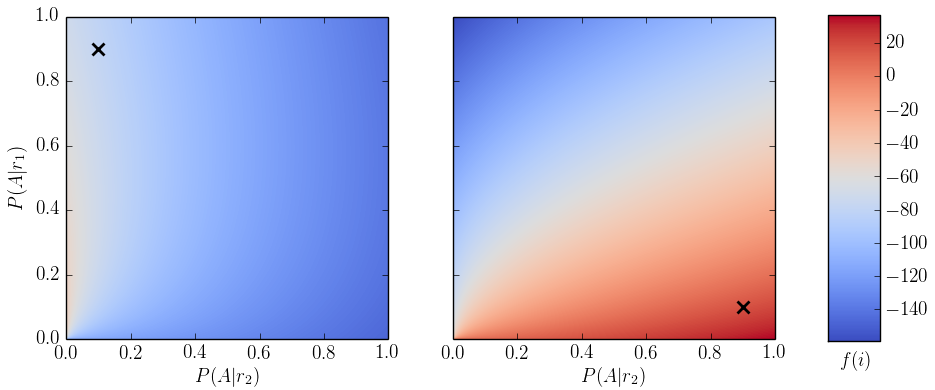
\includegraphics[width=\textwidth]{objective_function_cropped.png}
\caption{$f(i)$ with respect to partner $j$ (marked) in a two-referent language game, with $cost_A=80$, $cost_{r_1}=60$, $cost_{r_2}=120$, and $S=85$.}
\label{fig:1}
\end{figure}

There are a few issues to note with this formulation of $f$. Because the value of $f$ is dependent not only on the speaker's strategy, but also on the strategy their partner uses, because these strategies are a direct result of the positions of particles within the particle swarm, and because the positions of particles may change on every iteration of the PSO task, $f$ is \textit{extremely} dynamic. This dynamism is illustrated in \autoref{fig:1}. Particle swarm optimization is well-known for its resilience to dynamic functions, when accommodations are made by changing the methods by which particle velocities and best positions are updated \citep{engelbrecht2005}. However, the established accommodation techniques as presented in \cite{engelbrecht2005} are unsuitable for use here because they universally assume an objective function which updates periodically, not constantly. 
\marginpar{\textit{Is it appropriate to mention coevolution/niching in methods, should this be saved for the discussion, or is the treatment in \autoref{sec:pso_prev_work} sufficient?}}
Further, many of the techniques proposed make assumptions that would be implausible within the context of the \citeauthor{rohde2012} language game. For example, one technique is to reinitialize all or part of the particle swarm when the objective function changes, however, this would not only result in participants randomly changing strategies every iteration, but would be difficult to justify from a real-world perspective. In another technique, the associated scores for personal best and global best positions are recalculated when the objective function changes. However, in the context of the language game, this would be equivalent to allowing participants to continuously re-evaluate previously held strategies against their partner's current strategy. Because no appropriate adaptations for dynamic fitness functions were found, the implementation of PSO used was not altered to accommodate $f$.

\subsection{Model parameter optimization}
To complete the models described above, the model parameters were optimized to best fit the experimental data. These parameters included the standard PSO parameters, namely, the cognitive and social components, which were restricted to the interval $[0,4]$, an inertial dampening factor, which was restricted to the interval $[1,1.1]$, and an initial inertia, which was restricted to $[0,4]$. Additionally, a velocity dampening constant, which was used in the calculation of particle positions and was restricted to $[0,2]$, and the number of iterations over which the model was to be run, as restricted to $[100,1000]$, were also optimized.

Optimization of these parameters was itself performed via PSO over a $6$-dimensional search space. The parameter values used for this meta-optimization task were those recommended in \cite{shi1998} and \cite{solnon2010}. Parameters were optimized over $1255$ iterations of the particle swarm algorithm for the ``repair" model; these parameters were then also applied to the ``rejection" model. The optimization task itself utilized the unbounded ``rejection" technique as recommended in \cite{engelbrecht2005}. Initial particle positions were assigned using the randomized nonuniform method presented in \cite{mitchell1991}.

The parameter optimization task sought to minimize the discrepancy in rates of ambiguous form coordination, unambiguous form coordination, and failure to coordinate between the model and the experimental data, across all language game variants. In order to evaluate this, pairs were considered to have coordinated if, when the PSO task had completed, referents could be successfully communicated between the pair $\geq 95\%$ of the time.


\section{Results}
\subsection{Meta-optimization task (PSO parameters)}
\marginpar{\textit{Is there anything in particular that needs to be said about these here (as opposed to in the discussion)?}}
\begin{center}
    \begin{tabular}{ l l l r }
    Parameter & Optimized & Standard & $\% \Delta$ \\ \hline
    Cognitive component       & $0.689$ & $2.0$   & $-65.55\%$ \\ \hline
    Social component          & $2.897$ & $2.0$   & $+44.86\%$ \\ \hline
    Inertial dampening factor & $1.027$ & $1.001$ & $+2.58\%$\\ \hline
    Initial inertia           & $0.658$ & $1.2$   & $-45.17\%$ \\ \hline
    Velocity dampening factor & $1.202$ & N/A     & N/A\\ \hline
    Iterations                & $305$   & N/A     & N/A\\ 
    \end{tabular}
\end{center}

\subsection{Comparison of models to experimental data}
Results for both the rejection and repair models are compared against a baseline model, which makes use of the standard parameters used in the meta-optimization task. For each model, 250 simulations of 10 pairs were performed. Costs from each experiment as taken from the \citeauthor{rohde2012} studies are presented below.
\begin{center}
    \begin{tabular}{ l r r r }
     & $cost_{r_1}$ & $cost_{r_2}$ & $cost_{r_3}$ \\ \hline
    Experiment 1 & $60$ & $120$ & $280$ \\ \hline
    Experiment 2 & $60$ & $120$ & $250$ \\ \hline
    Experiment 3 & $80$ & $140$ & $165$ \\ \hline
    Experiment 4 & $80$ & $135$ & $170$ \\ 
    \end{tabular}
\end{center}

\textit{The results ended up seeming much harder to interpret than when I originally presented them to you. I'll bring my data for our next meeting, in the meanwhile, I've included graphs below, along with my questions/concerns where appropriate.}

\begin{center}
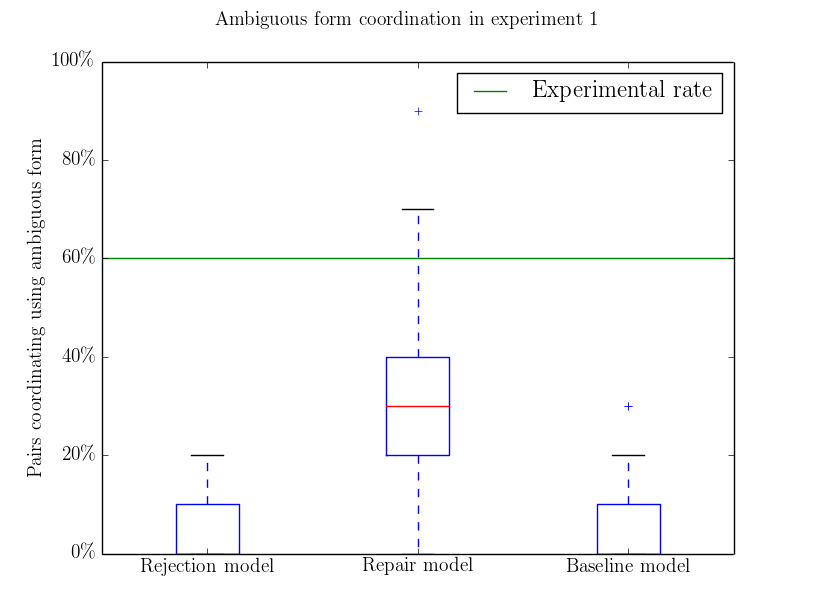
\includegraphics[width=\textwidth]{ambi_coord_exp1.png}
\textit{Is there a more cohesive way of presenting these? Should these box/whisker plots in particular perhaps be moved to an appendix?}
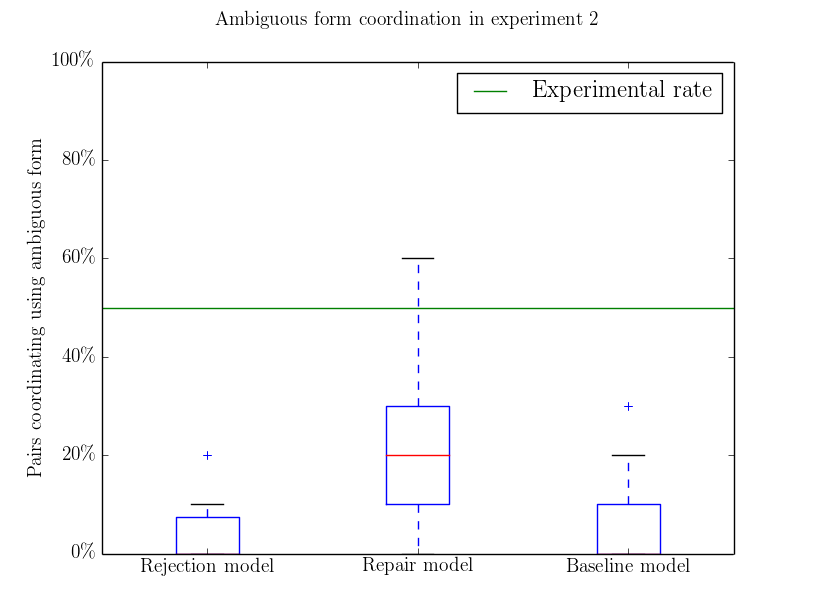
\includegraphics[width=\textwidth]{ambi_coord_exp2.png}
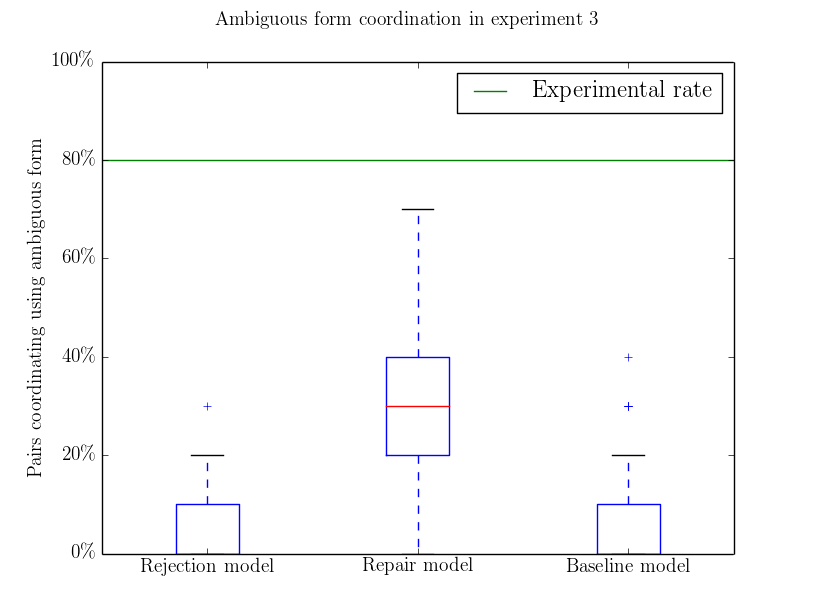
\includegraphics[width=\textwidth]{ambi_coord_exp3.png}
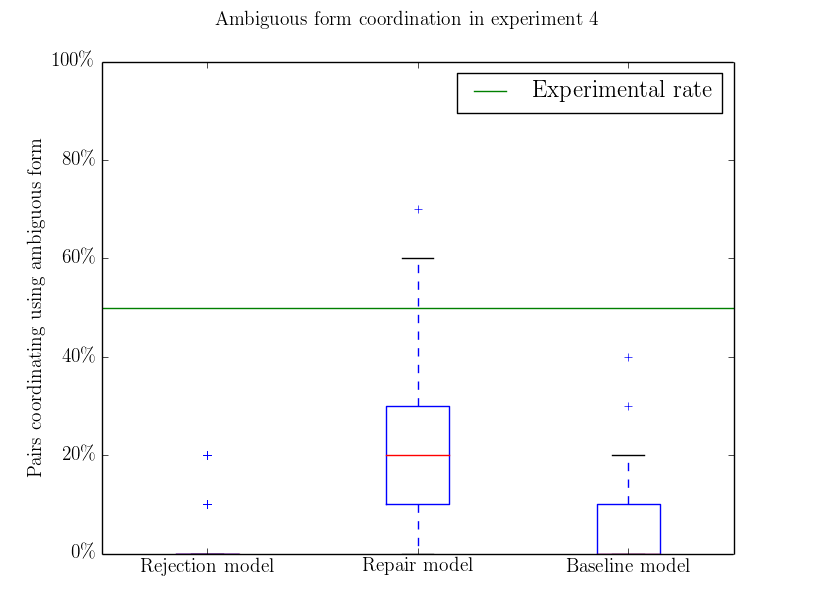
\includegraphics[width=\textwidth]{ambi_coord_exp4.png}
\end{center}

\begin{center}
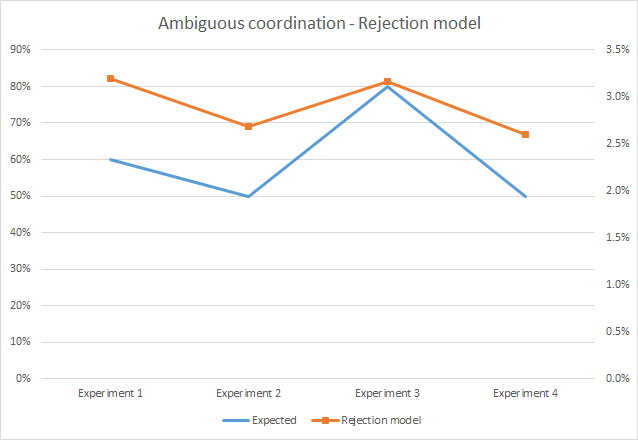
\includegraphics[width=\textwidth]{ambiguous_coordination_rejection.png}
\textit{Given that these are all at different scales, is there a way to present them together for comparison? How to choose/justify the scaling?}
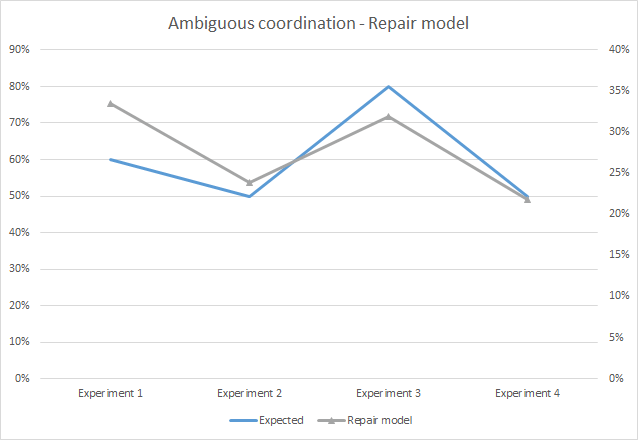
\includegraphics[width=\textwidth]{ambiguous_coordination_repair.png}
\marginpar{\textit{Would a bar chart be the best way to present this?}}
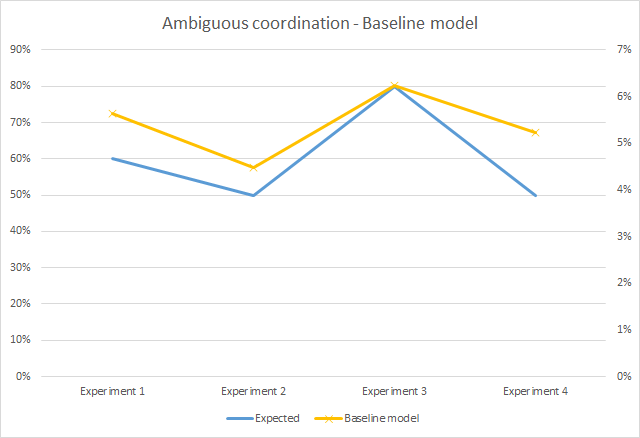
\includegraphics[width=\textwidth]{ambiguous_coordination_baseline.png}
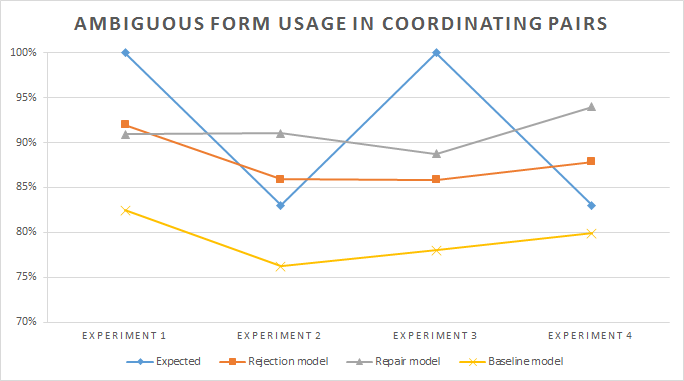
\includegraphics[width=\textwidth]{ambiguous_vs_unambiguous_smaller.png}
\textit{What is the most appropriate way to measure whether either of the two optimized models tracks the experimental data more effectively than the baseline model?}
\end{center}

\subsection{Predictions from successful model}
\textit{No longer clear which should be considered ``successful".}

\section{Discussion}
\begin{itemize}
\item Perhaps mention coevolutionary aspect here?

\item Model has response in keeping with experimental data without agents performing complex modeling (i.e. general optimization is sufficient to produce effects)

\item Repercussions of predictions

\item Possibility of applying PSO to other language games / experiments

\end{itemize}
\section{Conclusion}



\bibliographystyle{apacite}
\bibliography{dissertation.bib}


\end{document}
